%ब

\section{Solution 1:  Metadata with Special Characters}
\label{s:Implementation-Solution1} 

In Solution 1,  metadata is saved as a part of the entity in the
\texttt{Metadata} column. Whenever an operation on an entity triggers a
referential integrity validation, the metadata of the entity needs to be
retrieved, processed and accessed to perform validations. The way to retrieve,
process and access  metadata from the \texttt{Metadata} column in this solution 
is described in
% Section~\ref{ss:MD-Retrieval-Sol1}. The way the metadata is accessed is
% described in Section~\ref{ss:MD-Access-Sol1}
the following sections.

\subsection{Metadata Retrieval/Extraction/Processing}
\label{ss:MD-Retrieval-Sol1}

 Every time an operation is invoked on an entity its
metadata is accessed from its \texttt{Metadata} column and loaded as text. Since
the metadata for an entity holds all of its relevant constraints , each
constraint and its different parts are extracted from the text prior to the
validation.
Whenever an operation is invoked on an entity, its metadata is read as a String
by the \texttt{AbstractEntity} and the String is parsed to extract the values
of the constraints. All the special characters used within the
metadata are the delimiters for the String parsing. Following are the delimiters
used for parsing.
		\begin{itemize}
		  \item Special characters '\texttt{\{}', '\texttt{\}}' and '\texttt{;}' are
		  the delimiters for extracting each constraint from the metadata.
		  \item Special character '\texttt{;}' is the delimiter for identifying each
		  part within a constraint.
		  \item Special character '\texttt{:}' is the delimiter for extracting the
		  field name and the value of each part of the constraint.
		\end{itemize}
		
The experimental \ac{API} provides an entity class named \texttt{Metadata} which
extends the \texttt{AbstractEntitiy}. \texttt{Metadata} has the required getter
and setter access methods and stores the various parts of constraints as its
attributes which are maintained  during an operation . An example of the
\texttt{Metadata} entity class is shown in Figure~\ref{fi:MetadataEntityClass}.

	\begin{figure}[h] \centering
				% 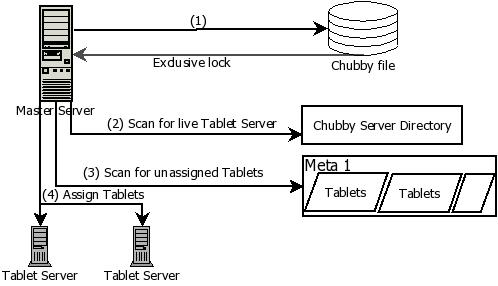
\includegraphics[width=5cm,   height=5cm]{. /figure/random. jpg}
		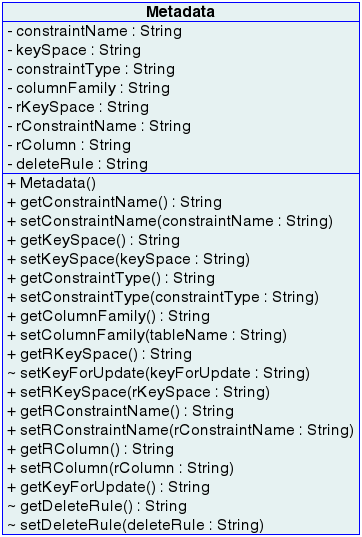
\includegraphics[width=0.5\textwidth]{./figure/Solutions/MetadataEntityClassOnly.png}
		\caption{Metadata Entity Class}\label{fi:MetadataEntityClass}
	\end{figure}
	
After parsing and extracting the values of the metadata, the
\texttt{AbstractEntity} 
sets the tokenized values as the attributes of \texttt{Metadata} using the 
setter methods. 

Since  metadata is present as the value in every super column, retrieving
 metadata  of a column family  does not require any additional  
connections to other column families in the keyspace. Moreover, the embedded
metadata storage is replicated across the cluster making metadata easily
accessible by every node in the cluster along with the column families.	 
	 
	 
\subsection{Metadata Access} \label{ss:MD-Access-Sol1}

After retrieving and processing the metadata for an entity, the constraint
values are set as the attributes of the \texttt{Metadata} entity class as explained above and
are available for access.
These values are accessed by the \texttt{ValidationHandler} whenever an
operation on the entity triggers a referential integrity validation. 

To perform  such validations, the \texttt{ValidationHandler} accesses the
relevant values of the constraints of an entity, using the getter
methods of the \texttt{Metadata} entity class.
For instance, to get the \texttt{DeleteRule} of a constraint applied on an
entity, \texttt{ValidationHandler} uses the \texttt{getDeleteRule()} method of
the \texttt{Metadata} entity class and similarly other  getter methods
are used to access the various parts of the constraint.
	 
The logic for the referential integrity validation by the
\texttt{ValidationHandler} once the  metadata is retrieved, parsed and accessed
is the same as described in Section~\ref{ss:VH}.

 

% The \ac{API} parses the metadata of an entity by reading any of its instances
% and need not load metadata from any external location.

% On the other hand,  the metadata for an entity would be the same for all its
% instances .  For example,  in the University example,  the metadata information
% for the \texttt{Student} entity is applicable to each of its instances, 
% indicating that each instance  should have a primary key called
% \texttt{StudentID}.
% Similarly,  all \texttt{Course} instances have the same \ac{PK} constraints
% applied on it.  When metadata is saved as a part of the  value, every instance
% of an entity will contain the constraint information in it's value.  Since the
% metadata information and constraints are same for all the instances of a single
% entity ,  this metadata is repeated every time an instance of the entity is
% inserted.  For example,  if \texttt{1000} \texttt{Student} instances are
% inserted,  the metadata for these \texttt{1000} instances are saved
% \texttt{1000} times too, along with these instances.  But the metadata is
% exactly same for all the instances \todo{(Figure~\ref{})}.


% The distributed nature of cloud \ac{NoSQL} \acp{DBMS} also means that the
% metadata is not only repeated several times within the same column family, 
% but also across the nodes in the cluster, thus increasing the redundancy of
% the metadata.  But such a redundancy and consumption of space to store the
% metadata is not a potential issue in cloud column-oriented key-value
% \acp{DBMS}, since storage on the cloud is inexpensive and  does not affect the
% economic benefits.
%  Such a storage mechanism is not expected to affect the efficiency of the
% cluster negatively as the metadata information is not large in size and is
% easily replicated along with the actual data and does not exert any extra
% resources in the cluster.  The performance of this solution is analysed  in
% Chapter~\ref{}.
%  Much research has been done in the area of  metadata management in
% distributed environments,  where emphasis is laid on the synchronous updates
% of metadata storage as well as its efficient storage and access
% mechanisms(\todo{cite more} Hackl et al.  2010).
% In Hackl et al.  (2010),  metadata management is discussed in the context of
% huge file systems, where metadata is stored separately in a suitable \ac{DBMS}
% so that such file systems can be managed and administered efficiently without
% slowing them down.  To analyse which type of \ac{DBMS} was more suitable for
% such a metadata storage,  they conducted various experiments and concluded
% that key-value \acp{DBMS} were more efficient in terms of speed,  memory and
% resource consumption when compared to popular \acp{RDBMS}.  As a part of their
% experiments, they adopted an interesting approach to store metadata in a
% key-value \ac{DBMS} ,  namely Tokyo Cabinet,  a popular \ac{NoSQL} \ac{DBMS}
% that stores records as simple key-value pairs in data files. Unlike Cassandra,
% tokyoCabinet does not involve data types or columns and so on (\todo{cite}). 
% In their approach,  metadata about the file system used in their experiment is
% inserted as a value which is associated with a unique key and the different
% parts of the metadata are separated by semicolons (Hackl et al.  2010).
	